\documentclass[12pt]{article}

% Packages
\usepackage{lipsum}
\usepackage{setspace}
\usepackage{indentfirst}
\usepackage{geometry}
\usepackage[nonumberlist, toc]{glossaries}
\usepackage{graphicx}
\usepackage{caption}
\usepackage{subcaption}
\usepackage{tabularx}
\usepackage{booktabs}
\usepackage[numbered]{./latex/mcode}
\usepackage{enumitem}
\usepackage{xcolor}
\usepackage [autostyle, english = american]{csquotes}
\usepackage{fancyhdr}
\usepackage{amsmath}
\usepackage{cite}

% Formatting
\geometry{letterpaper, portrait, margin=.85in}

\pagestyle{fancy}
\lhead{MSXII Suspension Parameters}
\rhead{Midnight Sun Solar Car Team}

\MakeOuterQuote{"}

\begin{document}

% Title Ppage
\begin{titlepage}
	\vspace*{3cm}
	\centering
	
\includegraphics[width=.25\textwidth]{./LaTex/midnightSunLogoCircle.png}\par
	\vspace{1.5cm}
	{\scshape\LARGE Midnight Sun Solar Car Team \par}
	{\scshape\large University of Waterloo\par}
	\vspace{3.5cm}
	{\huge\bfseries FEA Boundary Conditions\par}
	\vspace{0.2cm}
	\large MSXII
	\vfill
	Prepared by:\par
	Devon Copeland\par
	\vspace{1cm}
	\today\par
\end{titlepage}

% Main Matter
\section{Background}
\subsection{Vehicle Design}
Midnight Sun Twelve (MSXII) is a cruiser class, solar electric vehicle being designed with the goal of competing in the 2018 American Solar Challenge (ASC 2018) and the 2019 World Solar Challenge (WSC 2019). By definition, cruiser class solar vehicles must be multi-occupant and are designed with the intent of being more practical than a typical, challenger class solar car. Because of the unique requirements of this class, the spring rates and target damping coefficients on MSXII's suspension must be selected to optimize for efficiency while still keeping driver comfort in mind. This report proposes an analytical technique for determining the response of a suspension system to any given road conditions. 

\subsection{Important Vehicle Parameters}
Table \ref{tab:params} lists vehicle parameters that are of importance to the design and analysis of MSXII's suspension. The mass and moment of inertia was computed by CAD software. 
\begin{table}[htbp]
	\centering
	\caption{Important Vehicle Parameters}
	\label{tab:params}
	\begin{tabular}{lll}
	Mass ($M$)                            	& 550  & $kg$       \\
	Wheelbase                       	 	& 2.60  & $m$  		\\
	Track                       	 		& 1.60  & $m$  		\\
	Tire Diameter                       	 		& 0.53  & $m$  		\\
	Wheel Assembly Moment of Inertia ($J_w$)   	& 0.25  & $kgm^2$  		\\
	Distance from Front Wheel to CoG ($a$)	& 1.32 & $m$  		\\
	Distance from Road to CoG ($h$)		& 0.52 & $m$  		\\
	%Moment of Inertia Normal to Symmetry Plane at CoG ($I_{xx}$) & 550  & $kgm^2$ \\
	Full Wheel Travel in Compression 	& 45   & $mm$ 		\\
	Front Coilover Angle from Vertical	& 40   & $\circ$ 	\\
	Rear Coilover Angle from Vertical	& 30   & $\circ$
	\end{tabular}
\end{table}
\subsection{Suspension Architecture}
MSXII's front suspension comprises of a double wishbone linkage with an outboard coilover while the rear suspension comprises of independent trailing arms allowing for zero scrub and thus less rolling resistance. Figure \ref{fig:solidworksScreenshots} shows the screenshots of the front and rear suspension.  
\begin{figure}[htbp]
	\centering
    \begin{subfigure}[b]{.32\textwidth}
		\caption{Front Isometric View}
		\centering
        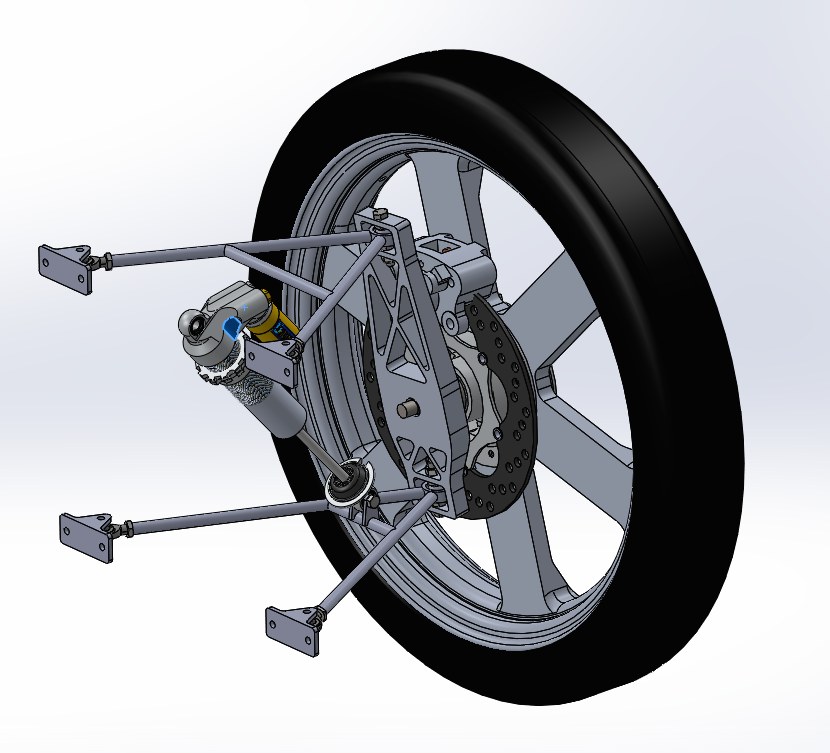
\includegraphics[height=3.5cm]{./LaTex/frontIso.PNG}
    \end{subfigure}
    \begin{subfigure}[b]{.32\textwidth}
		\caption{Rear Isometric View}
		\centering
        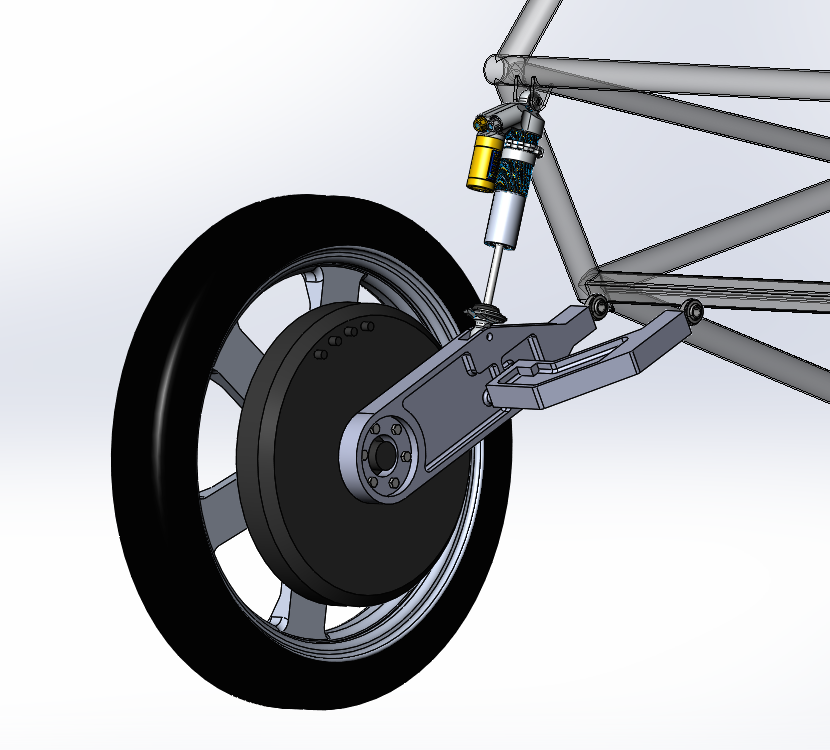
\includegraphics[height=3.5cm]{./LaTex/rearIso.PNG}
        \label{fig:c8}
    \end{subfigure}
    \begin{subfigure}[b]{.32\textwidth}
		\caption{Rear Sie View}
		\centering
        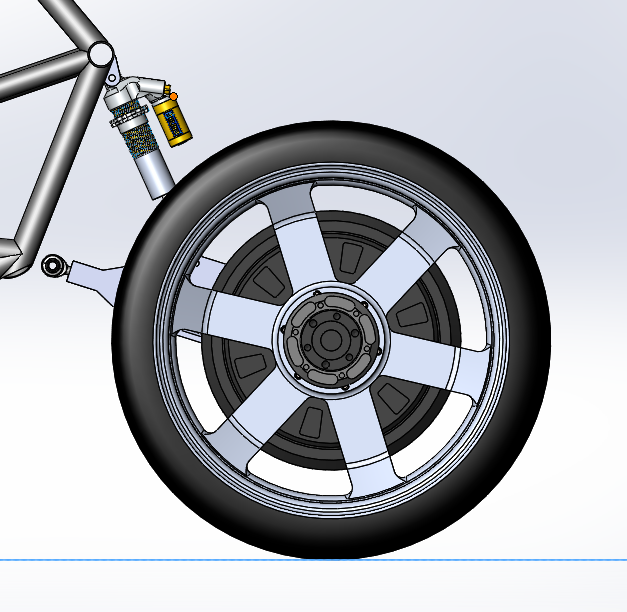
\includegraphics[height=3.5cm]{./LaTex/rearRight.PNG}
        \label{fig:c9}
    \end{subfigure}
    \caption{MSXII Suspension Design (Screenshots from Solidworks)}
	\label{fig:solidworksScreenshots}
\end{figure}
\subsection{Approach to FEA}
\textit{explain the different loading conditions to be tested (dynamic, static, fatigue etc.)}

\pagebreak
\section{Static Loading}
\label{sec:paramSelection}
Assuming a smooth driving surface, the largest normal force acting on the front tire will occur while braking in a turn. Similarly, the largest normal force acting on the rear tire will occur while accelerating in a turn. To approximate these loading condition, the a superposition of two static half car models is used; one for cornering and one for hard braking.  

\subsection{Hard Braking}
\label{sec:hardBraking}
\begin{figure}[h!]
	\centering
	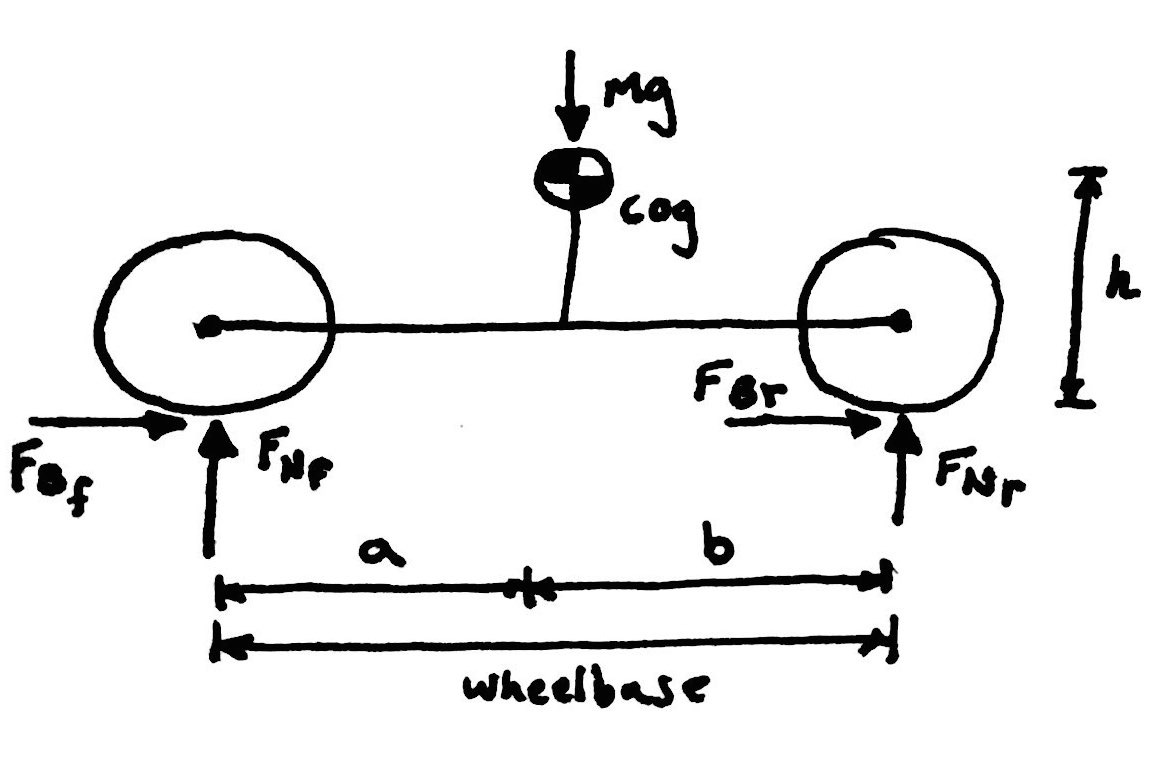
\includegraphics[width=.5\textwidth]{./LaTex/brakingFBD.jpg}
	\caption{Free Body Diagram of a Car Braking}
	\label{fig:barkingFBD}
\end{figure}
Figure \ref{fig:barkingFBD} shows a free body diagram of a half car model undergoing braking. MSXII will only have brake callipers on the front wheels however regenerative braking from the hub motors will also provide a braking force at the rear contact patches. Assuming a generous coefficient of static friction, $\mu _s$, of 1.0 and the extreme case where the both the font and rear tires are about to begin sliding, the combined braking force can be expressed as: 
\begin{equation}
	F_{braking} = F_{Nf} + F_{Nr} = \mu _s F_{N_{net}} =  \mu _s Mg = (1.0)(550kg)\left(9.81\frac{m}{s^2}\right) = 5.40kN
\end{equation}
From Figure \ref{fig:barkingFBD}, summing the moments about the centre of gravity and the vertical forces results in the following equations: 
\begin{equation}
	aF_{Nf} = hF_{braking} + bF_{Nr}
\end{equation}
\begin{equation}
	F_{Nf} + F_{Nr} = Mg
\end{equation}
Solving for the front normal force: 
\begin{equation}
\begin{split}
	aF_{Nf} &= hF_{braking} + b(Mg - F_{Nf})\\
	F_{Nf} &= \frac{hF_{braking} + bMg}{a+b} = \frac{(0.52m)(5.40kN)+(1.28m)(550kg)\left(9.81\frac{m}{s^2}\right)}{(1.32m)+(1.28m)} = 3.74kN
\end{split}
\end{equation}
Note that 3.74kN is for both front wheels. Therefore there is approximately \textbf{1.87kN} of normal force on each front tire during hard braking. 

\subsection{Maximum acceleration}
MSXII will use SCM-150s which have a peak torque of 135Nm, however from the manufacturer provided torque speed curves, a more reasonable upper limit to for peak torque sustainable as the car accelerates is approximately 100Nm \cite{scm}. From this torque value and a number of other vehicle parameters the vehicle's maximum acceleration can be calculated as follows: 

\begin{equation}
	a = \frac{F_w}{\frac{1}{2}M}
\end{equation}
\begin{equation}
	\alpha_w = \frac{T_m - F_wr}{J_w}
\end{equation}
\begin{equation}
	\alpha_w = ar
\end{equation}
where $a$ is the acceleration of the vehicle, $F_w$ is the friction force acting on a single tire while accelerating, $J_w$ is the moment of inertia of the wheel assembly, $r$ is the radius of the tire, $T_m$ is the torque from the motor and $\alpha_w$ is the angular acceleration of the wheel. 

Rearranging the above three equations, the acceleration of the vehicle can be expressed as a function of motor torque as follows: 
\begin{equation}
\begin{split}
	a &= \frac{T_m r}{\frac{1}{2}Mr^2 + J_w} \\
	a &= \frac{(100Nm)(0.27m)}{\frac{1}{2}(550kg)(0.27m^2)^2 + 0.25kgm^2} = 1.33m/s^2
\end{split}
\end{equation}
Solving for friction force on a single rear tire: 
\begin{equation}
	F_w = Ma = (550kg)(1.33m/s^2) = 732N
\end{equation}
Using the same approach as demonstrated in section \ref{sec:hardBraking}, the resulting normal force on the rear wheels can be calculated as follows: 
\begin{equation}
\begin{split}
	bF_{Nr} &= hF_{w} + a(Mg - F_{Nr})\\
	F_{Nr} &= \frac{hF_{w} + aMg}{a+b} = \frac{(0.52m)(732N)+(1.32m)(550kg)\left(9.81\frac{m}{s^2}\right)}{(1.32m)+(1.28m)} = 2.89kN
\end{split}
\end{equation}
Note that 2.88kN is for both rear wheels. Therefore there is approximately \textbf{1.44kN} of normal force on each rear tire during maximum acceleration.

\subsubsection{Cornering}
\begin{figure}[h!]
	\centering
	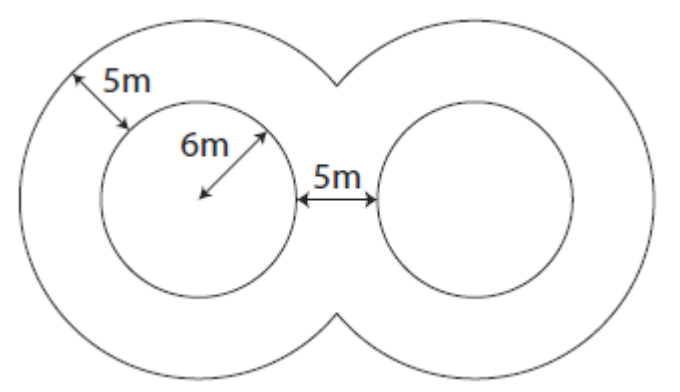
\includegraphics[width=.5\textwidth]{./LaTex/dynamicScrutineering.PNG}
	\caption{Figure of Eight Course from ASC 2018 Regulations 
	\cite{ASC2018regs}}
	\label{fig:dynamicScrutineering}
\end{figure}
To determine the lateral force subjected to the vehicle, the worst case of two scenarios is selected. The first scenario originates from the ASC 2018 regulations while the second draws its roots from actual highway geometry and speed limits. 

For the first scenario, the ASC 2018 regulations stipulate that a vehicle must be able to navigate a figure of eight as shown in Figure \ref{fig:dynamicScrutineering} in less than 18 seconds \cite{ASC2018regs}. Since the average arc length of the figure of eight is $34\pi m$, the net lateral force required to navigate the figure of eight can be found as follows:
\begin{equation}
	F_{si} + F_{so} = F_{steer} = \frac{Mv^2}{r} = \frac{(550kg)\left(\frac{34\pi m}{18s}\right)^2}{8.5m} = 2.28kN
\end{equation}

\begin{figure}[htbp]
	\centering
    \begin{subfigure}[b]{.4\textwidth}
		\caption{Conestoga Pkwy. \& Wellington St.}
		\centering
        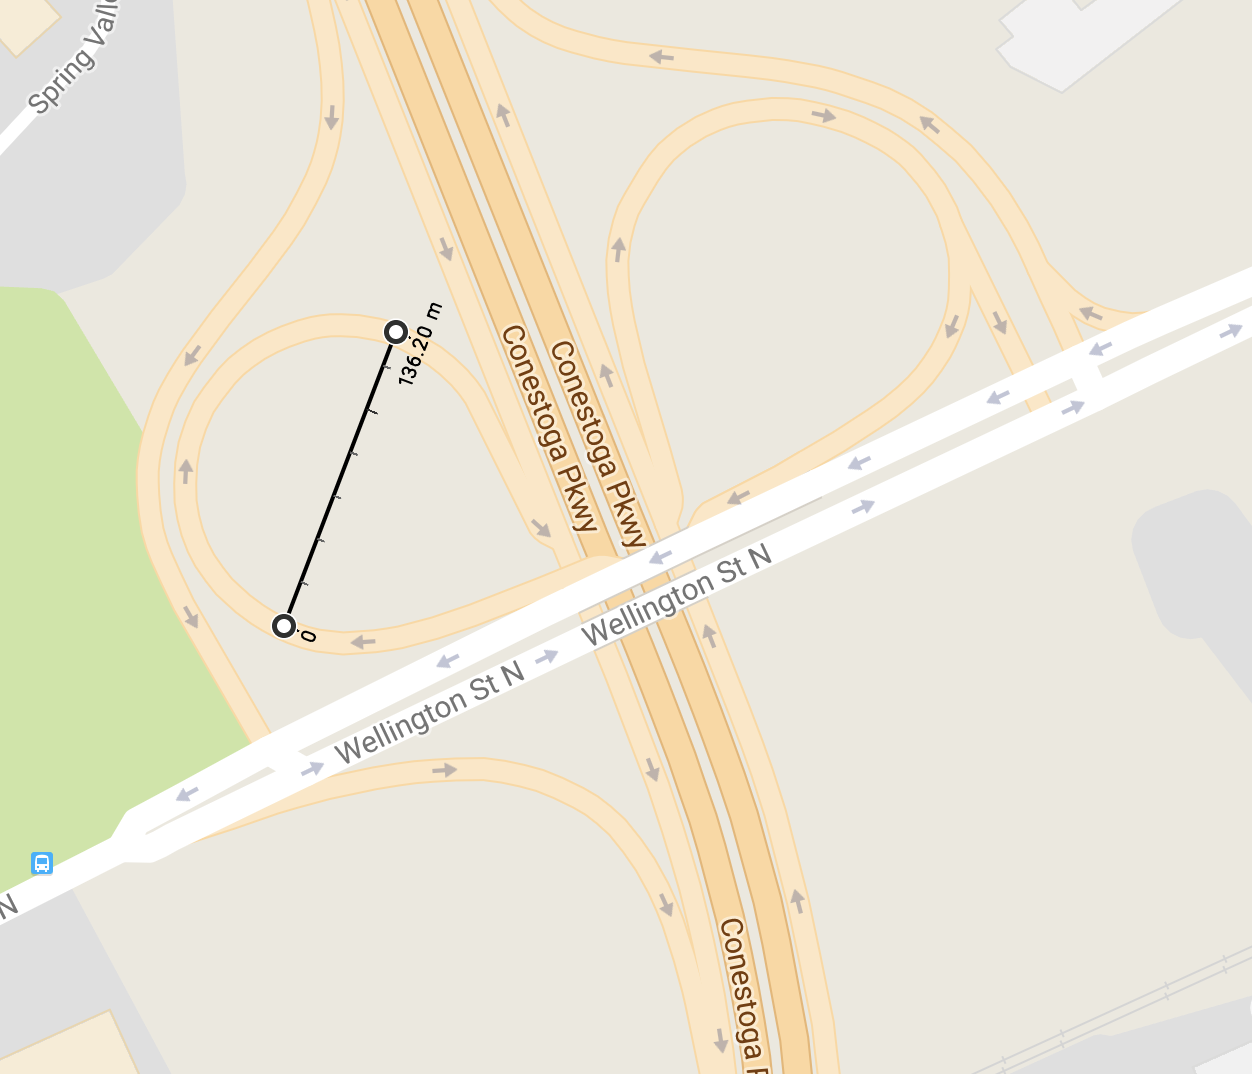
\includegraphics[height=4.5cm]{./LaTex/hw1.PNG}
    \end{subfigure}
    \begin{subfigure}[b]{.4\textwidth}
		\caption{Conestoga Pkwy. \& University Ave.}
		\centering
        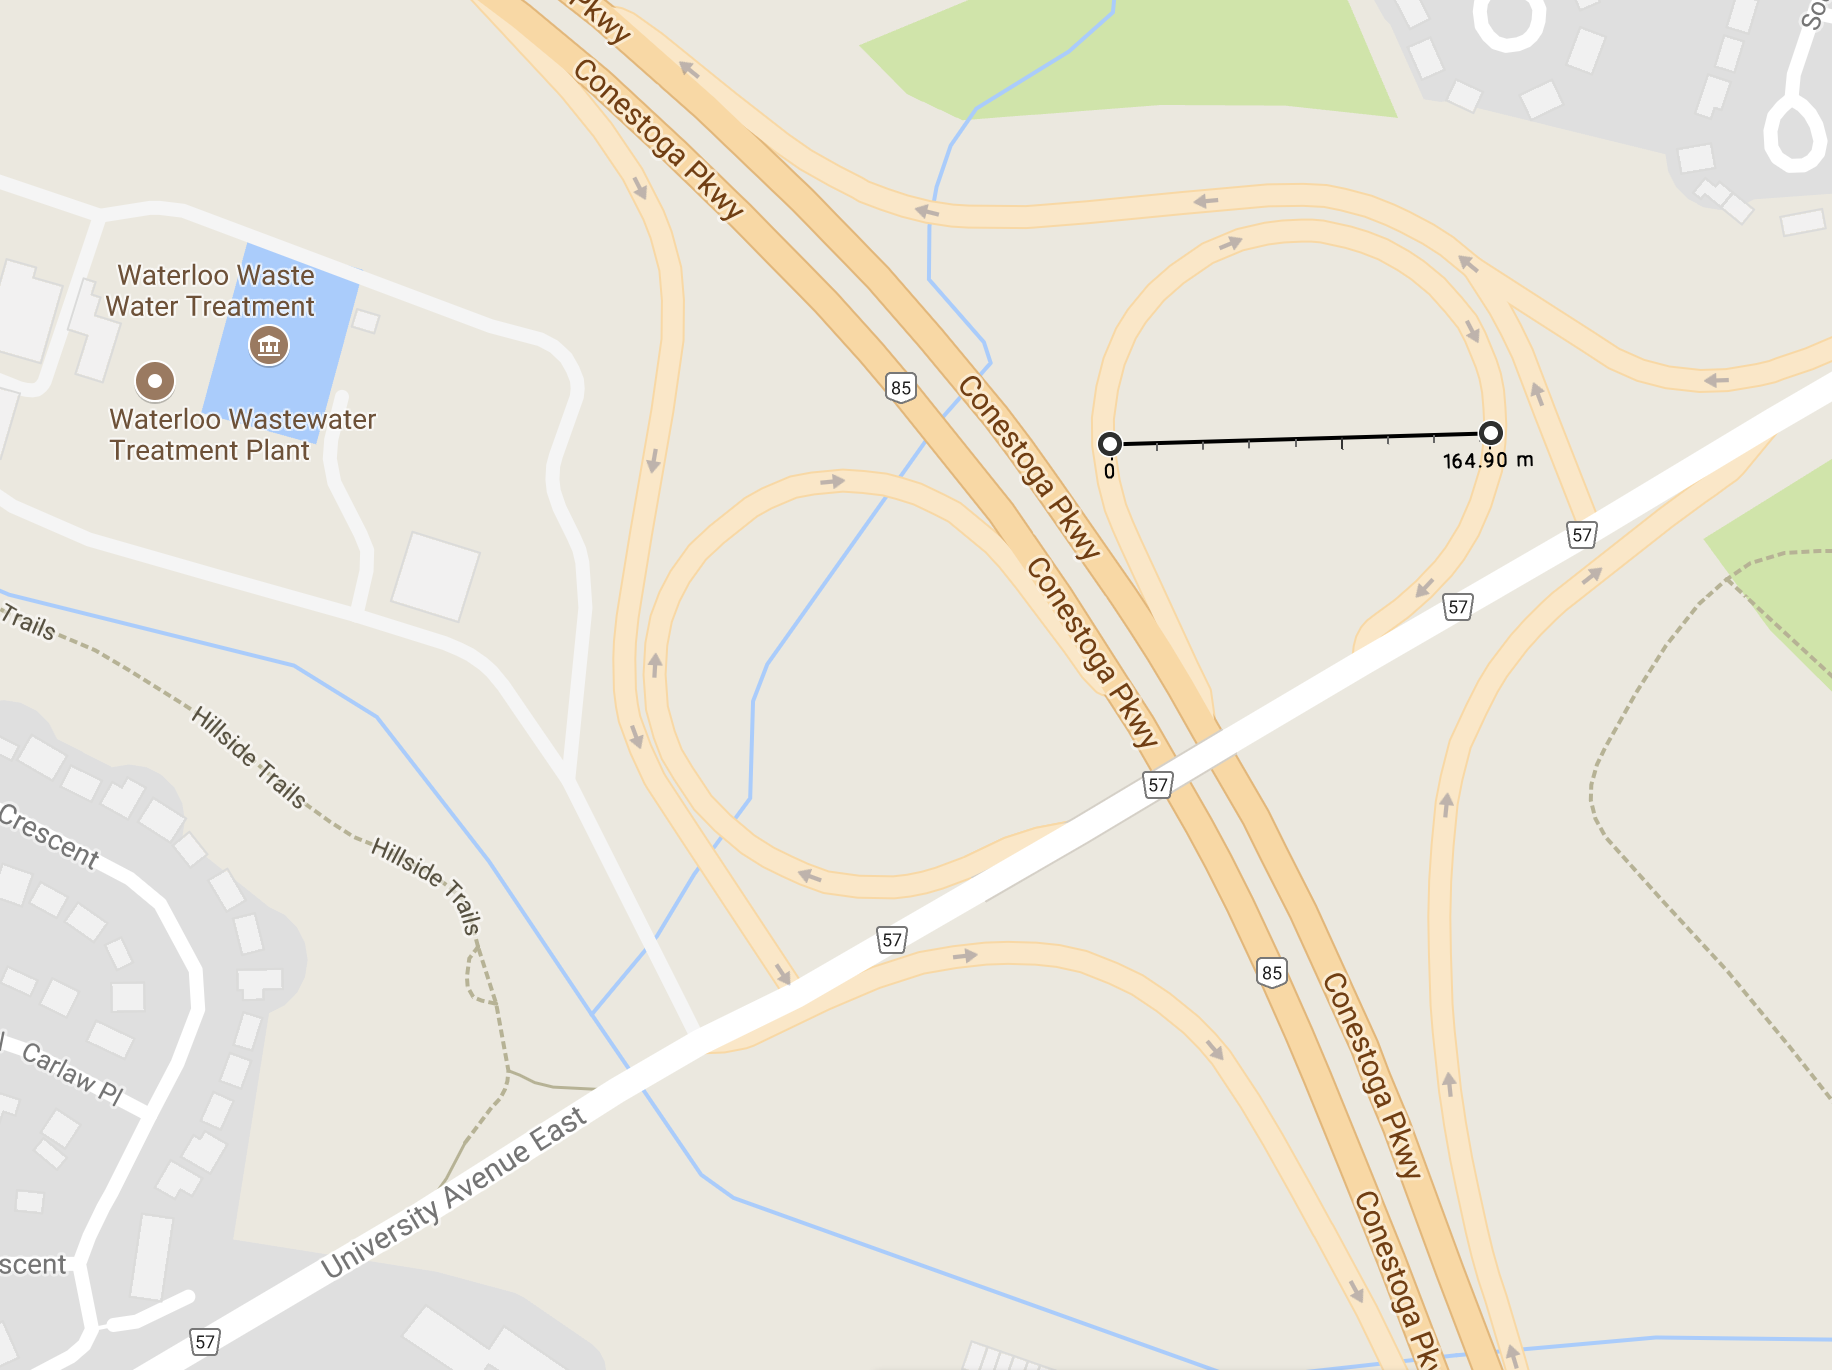
\includegraphics[height=4.5cm]{./LaTex/hw2.PNG}
    \end{subfigure}
    
    \bigskip
    \begin{subfigure}[b]{.4\textwidth}
		\caption{Conestoga Pkwy. \& King St.}
		\centering
        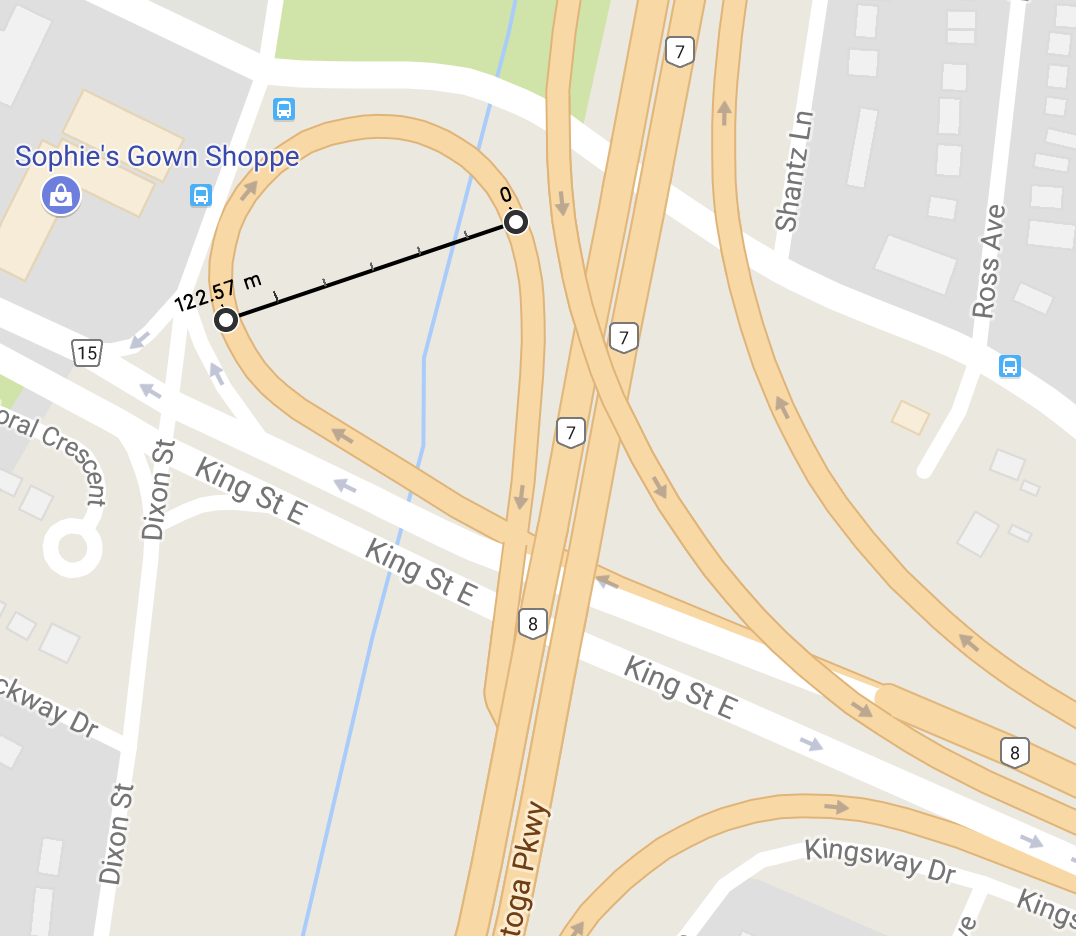
\includegraphics[height=4.5cm]{./LaTex/hw3.PNG}
    \end{subfigure}
    \begin{subfigure}[b]{.4\textwidth}
		\caption{Speed Limit on Conestoga Pkwy Exits}
		\centering
        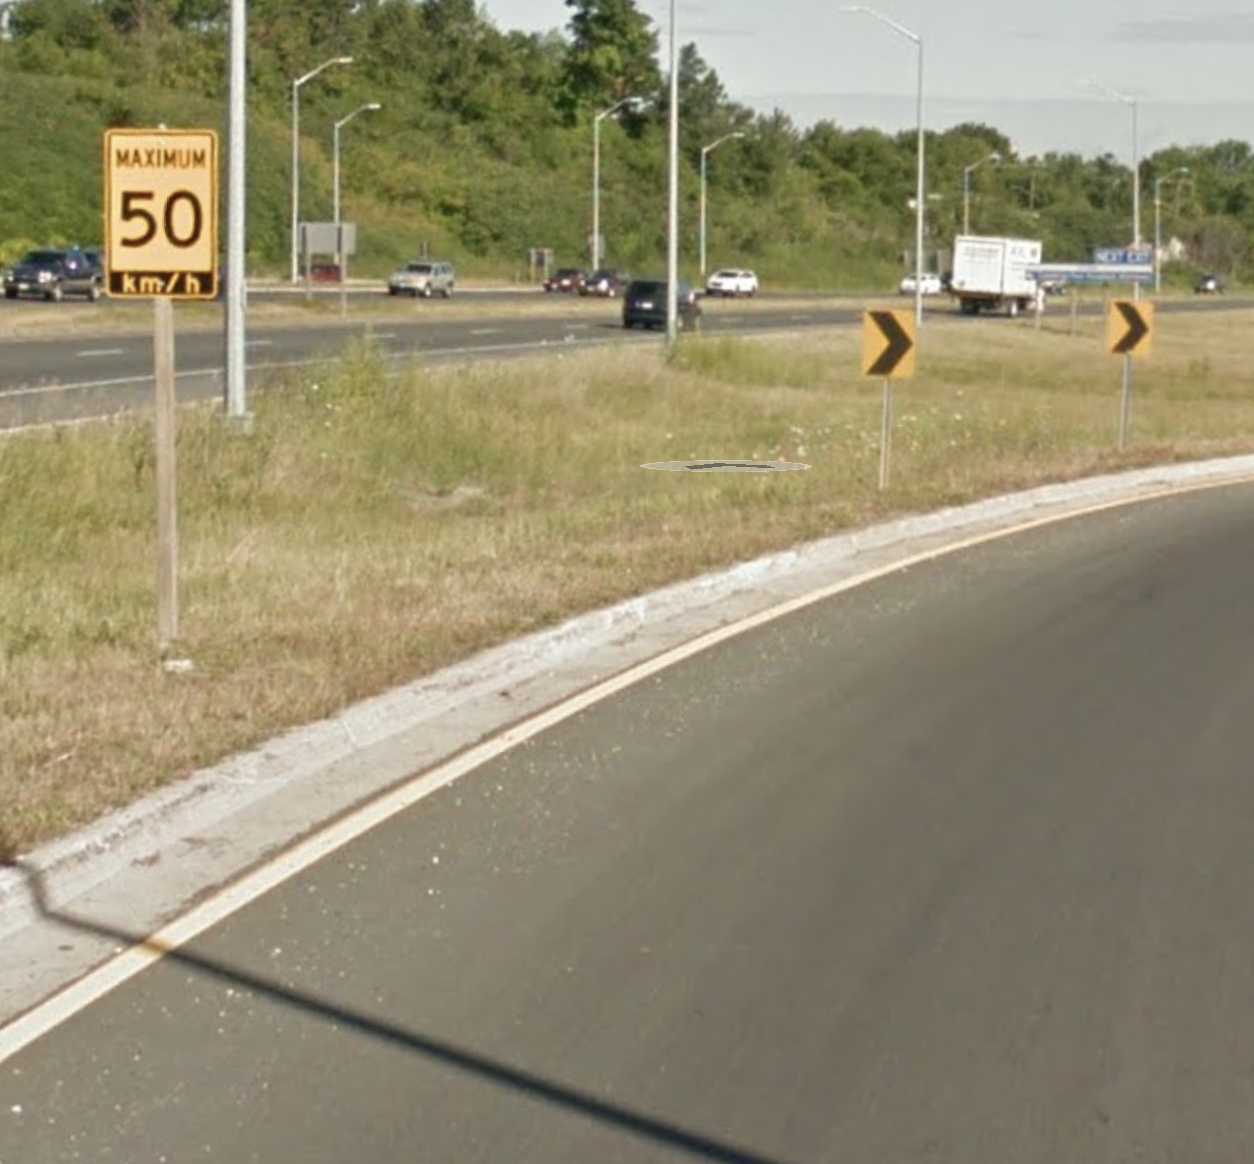
\includegraphics[height=4.5cm]{./LaTex/speedLimit.PNG}
    \end{subfigure}
    \caption{Highway Exist Around the University of Waterloo}
	\label{fig:highwayExits}
\end{figure}
For the second scenario, the diameter of several highway exit ramps around the University of Waterloo were measured as shown in Figure \ref{fig:highwayExits}. The recommended speed limit on these exits 50$km/hr$. Assuming a worst case scenario where the vehicle takes an exit with a 100$m$ diameter at 60$km/hr$ (16.67$m/s$), required lateral force required to navigate this corner can be found as follows: 
\begin{equation}
	F_{steer} = \frac{Mv^2}{r} = \frac{(550kg)(16.67m/s)^2}{50m} = 3.06kN
\end{equation}

Since the lateral force required in the second scenario is highest, 3.06kN will be used as the worst case cornering force. 

\begin{figure}[h!]
	\centering
	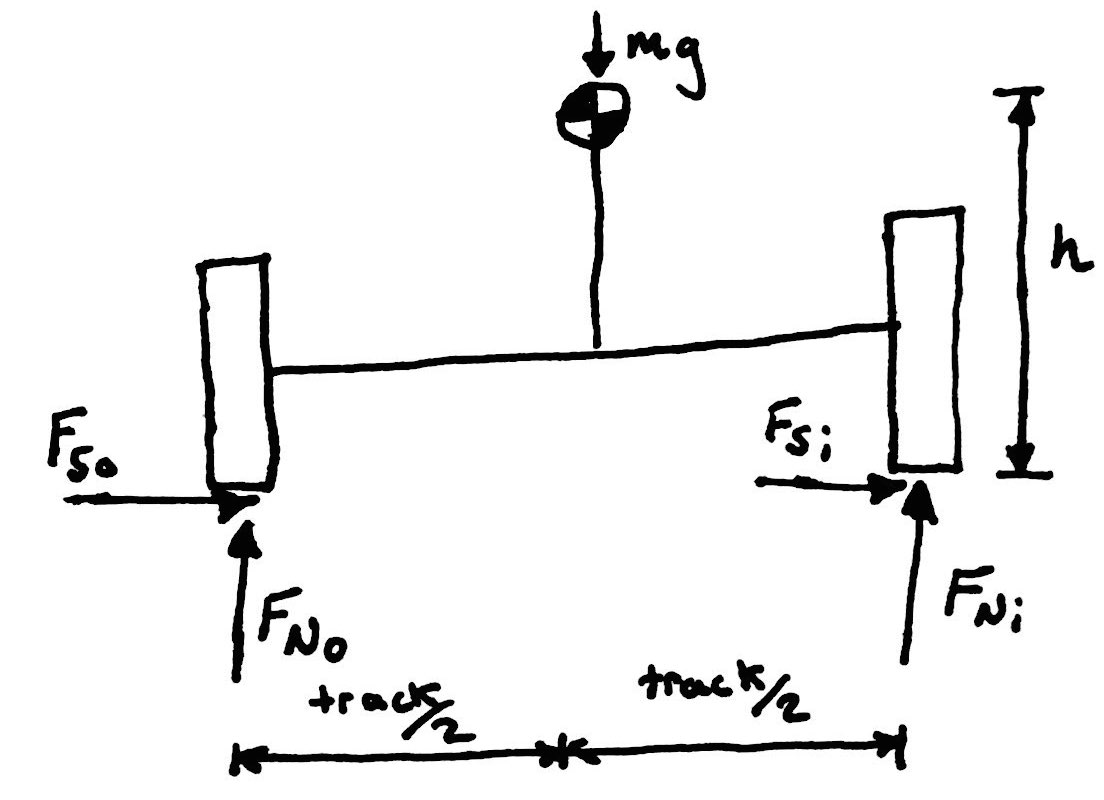
\includegraphics[width=.5\textwidth]{./LaTex/steerFBD.jpg}
	\caption{Free Body Diagram of a Car Cornering}
	\label{fig:steerFBD}
\end{figure}

Using the half car model shown if Figure \ref{fig:steerFBD}, summing the moments about the centre of gravity and the vertical forces results in the following equations: 
\begin{equation}
	\frac{track}{2}F_{No} = hF_{steer} + \frac{track}{2}F_{Ni}
\end{equation}
\begin{equation}
	F_{No} + F_{Ni} = Mg
\end{equation}
Solving for the outside wheel normal force: 
\begin{equation}
\begin{split}
	\frac{track}{2}F_{No} &= hF_{steer} + \frac{track}{2}(Mg - F_{Ni})\\
	F_{No} &= \frac{hF_{steer} + \frac{track}{2}Mg}{track} = \frac{(0.52m)(3.06kN)+(0.80m)(550kg)\left(9.81\frac{m}{s^2}\right)}{1.60m} = 3.69kN
\end{split}
\end{equation}
Solving for the inside wheel normal force: 
\begin{equation}
	F_{Ni} = Mg - F_{No} = (550kg)\left(9.81\frac{m}{s^2}\right) - 3.69kN = 1.71kN
\end{equation}
Note that the forces above are for both front and rear outside wheels. Assuming the force is evenly split between the front and rear, there is approximately \textbf{1.85kN} of normal force on each outside tire and \textbf{0.85kN} for each inside tire during maximum cornering.
 
\subsection{Superposition}
The braking accelerating and cornering conditions subject the wheels to normal forces that differ from those seen when the car is at rest. The change in normal force for each loading condition can be expressed as follows: 
\begin{equation}
	\begin{split}
		\Delta F_{Nf_{braking}} &= F_{Nf_{braking}} - \frac{Mg}{4} =  1.87kN - 1.35kN = 0.52kN\\
		\Delta F_{Nr_{accelerating}} &= F_{Nf_{braking}} - \frac{Mg}{4} =  1.44kN - 1.35kN = 0.09kN\\
		\Delta F_{No_{cornering}} &=  F_{No_{cornering}} - \frac{Mg}{4} =  1.85kN - 1.35kN = 0.50kN \\
		\Delta F_{Ni_{cornering}} &=  F_{No_{cornering}} - \frac{Mg}{4} =  0.85kN - 1.35kN = -0.50kN
	\end{split}
\end{equation}
To approximate the worst case loading condition, a superposition of the changes in normal force and the nominal normal force is applied. Note that the nominal force used is the same for each wheel which assumes a centre of gravity approximately centred along the wheelbase.   
\begin{equation}
	\begin{split}	
	F_{Nfi_{max}} = \Delta F_{Nf_{braking}} + \Delta F_{Ni_{cornering}} + F_{N_{nominal}} = 0.52kN - 0.50kN + 1.35kN = 1.24kN \\
	F_{Nfo_{max}} = \Delta F_{Nf_{braking}} + \Delta F_{No_{cornering}} + F_{N_{nominal}} = 0.52kN + 0.50kN + 1.35kN = 2.37kN \\
	F_{Nri_{max}} = \Delta F_{Nr_{braking}} + \Delta F_{Ni_{cornering}} + F_{N_{nominal}} = 0.09kN - 0.50kN + 1.35kN = 0.94kN \\
	F_{Nro_{max}} = \Delta F_{Nr_{braking}} + \Delta F_{No_{cornering}} + F_{N_{nominal}} = 0.09kN + 0.50kN + 1.35kN = 1.94kN 
	\end{split}
\end{equation}

\subsection{Summary}
Table \ref{tab:forcesSummary} summarizes the loading conditions used for static structural FEA simulations on the suspension and steering components. Note that the direction of the force corresponds's with the global coordinate system of the MSXII and the vectors shown in Figure \ref{fig:forcesSummary}. The assemblies shown are for the driver's side of the vehicle

\begin{table}[h!]
\centering
\caption{Summary of Suspension Loading Conditions}
\label{tab:summary}
\begin{tabular}{llll}
\textbf{Case}                                  & \textbf{Fx (kN)} & \textbf{Fy (kN)} & \textbf{Fz (kN)} \\
Braking \& Cornering (Inside Front Wheel)      & 1.53             & 1.24             & 2.70             \\
Braking \& Cornering (Outside Front Wheel)     & -1.53            & 2.37             & 2.70             \\
Accelerating \& Cornering (Inside Rear Wheel)  & 1.53             & 0.94             & 0.73             \\
Accelerating \& Cornering (Outside Rear Wheel) & -1.53            & 1.94             & 0.73            
\end{tabular}
\end{table}

\begin{figure}[h!]
	\centering
    \begin{subfigure}[b]{.48\textwidth}
		\caption{Font Suspension}
		\centering
        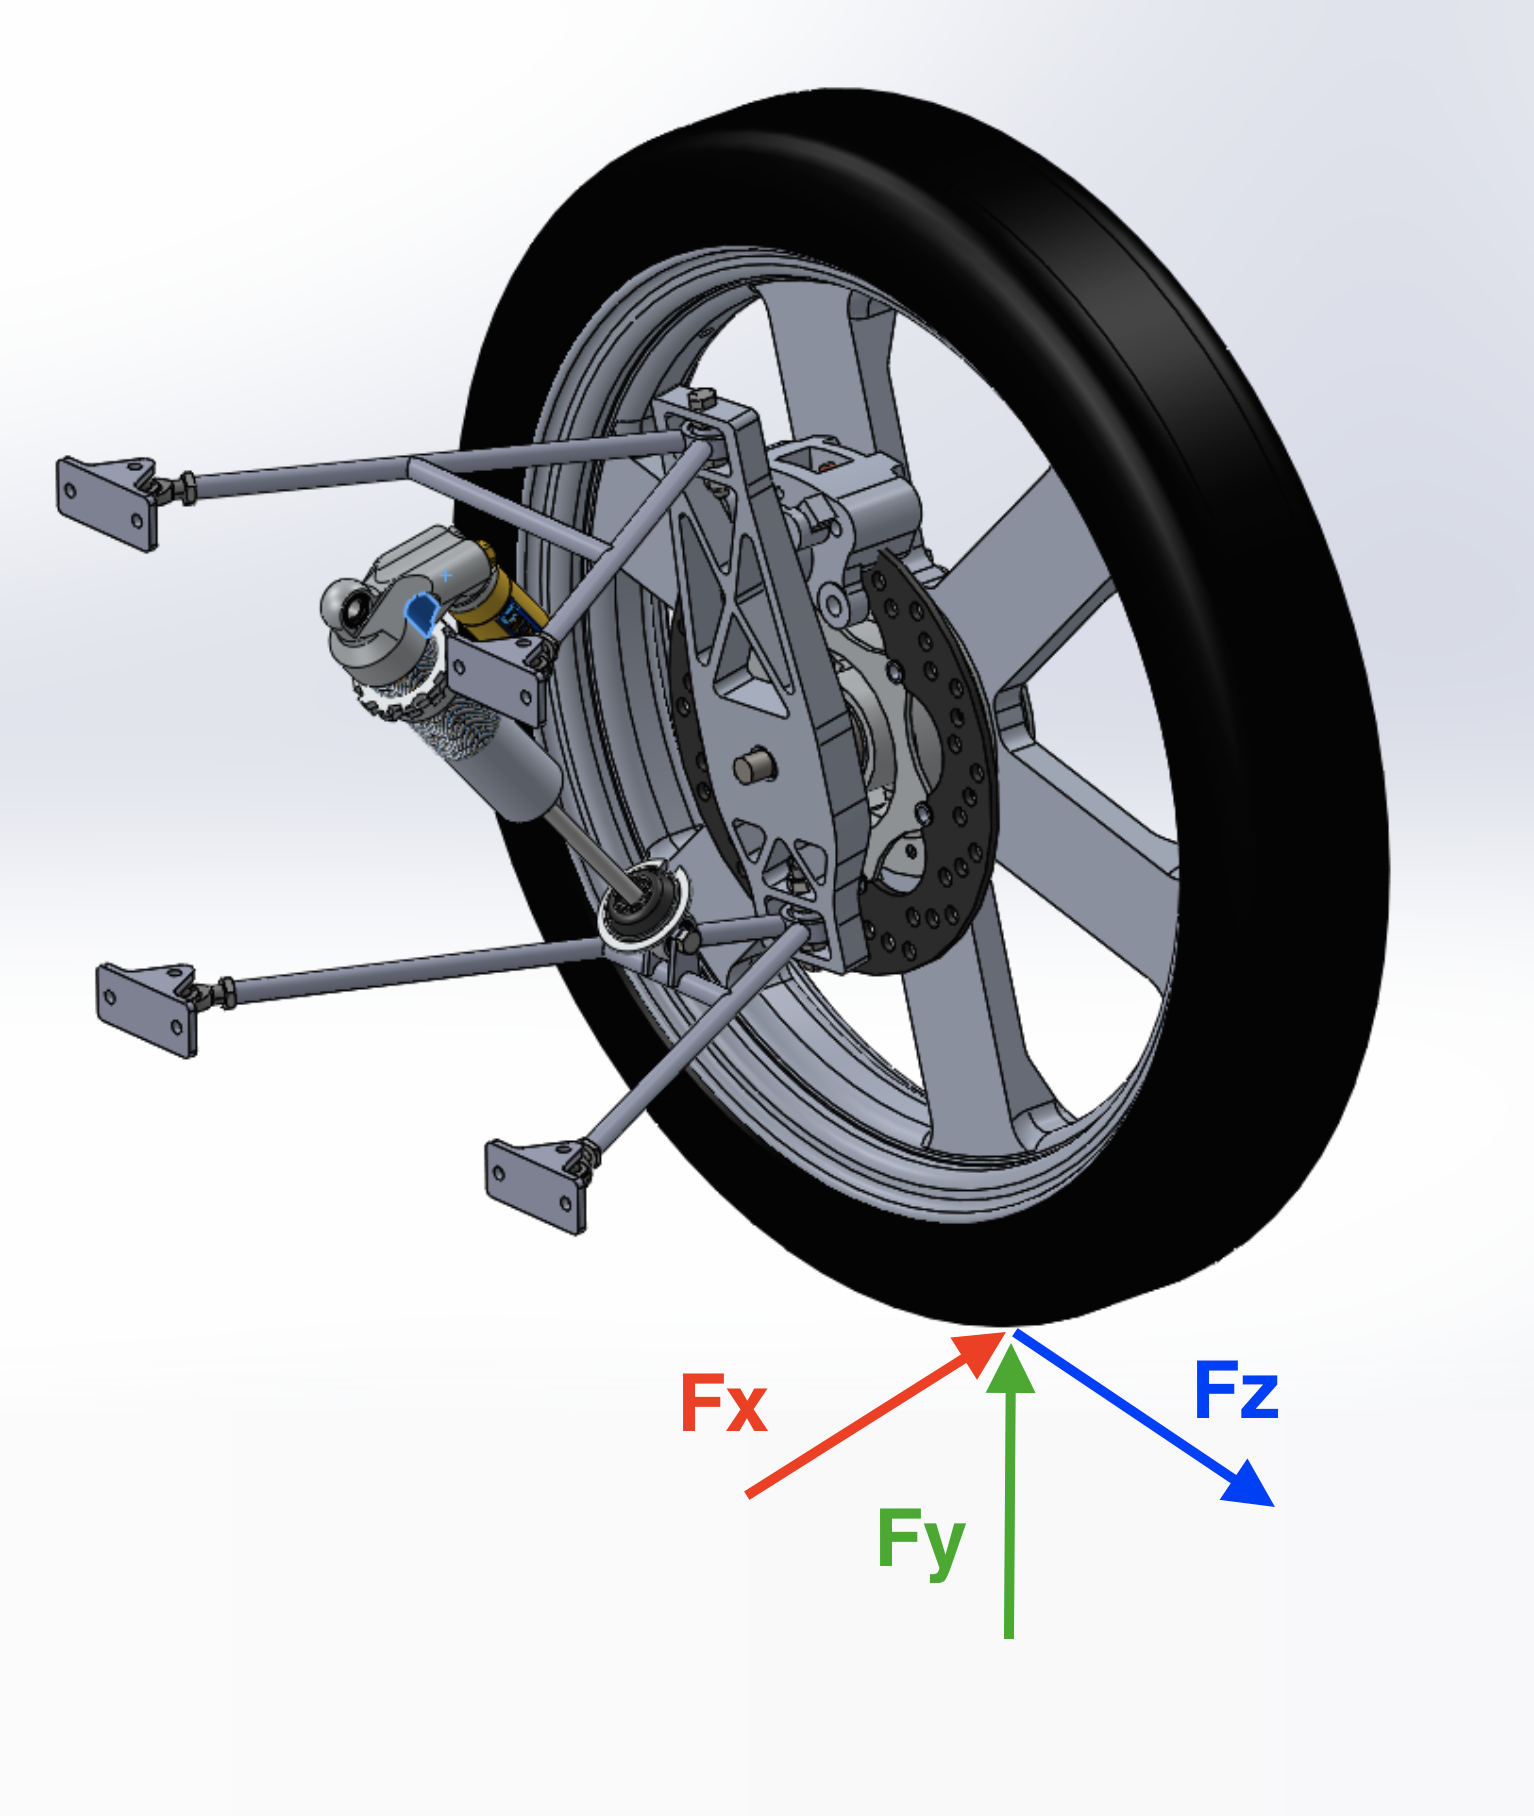
\includegraphics[height=9cm]{./LaTex/frontIsoForces.PNG}
    \end{subfigure}
    \begin{subfigure}[b]{.48\textwidth}
		\caption{Rear Suspenion}
		\centering
        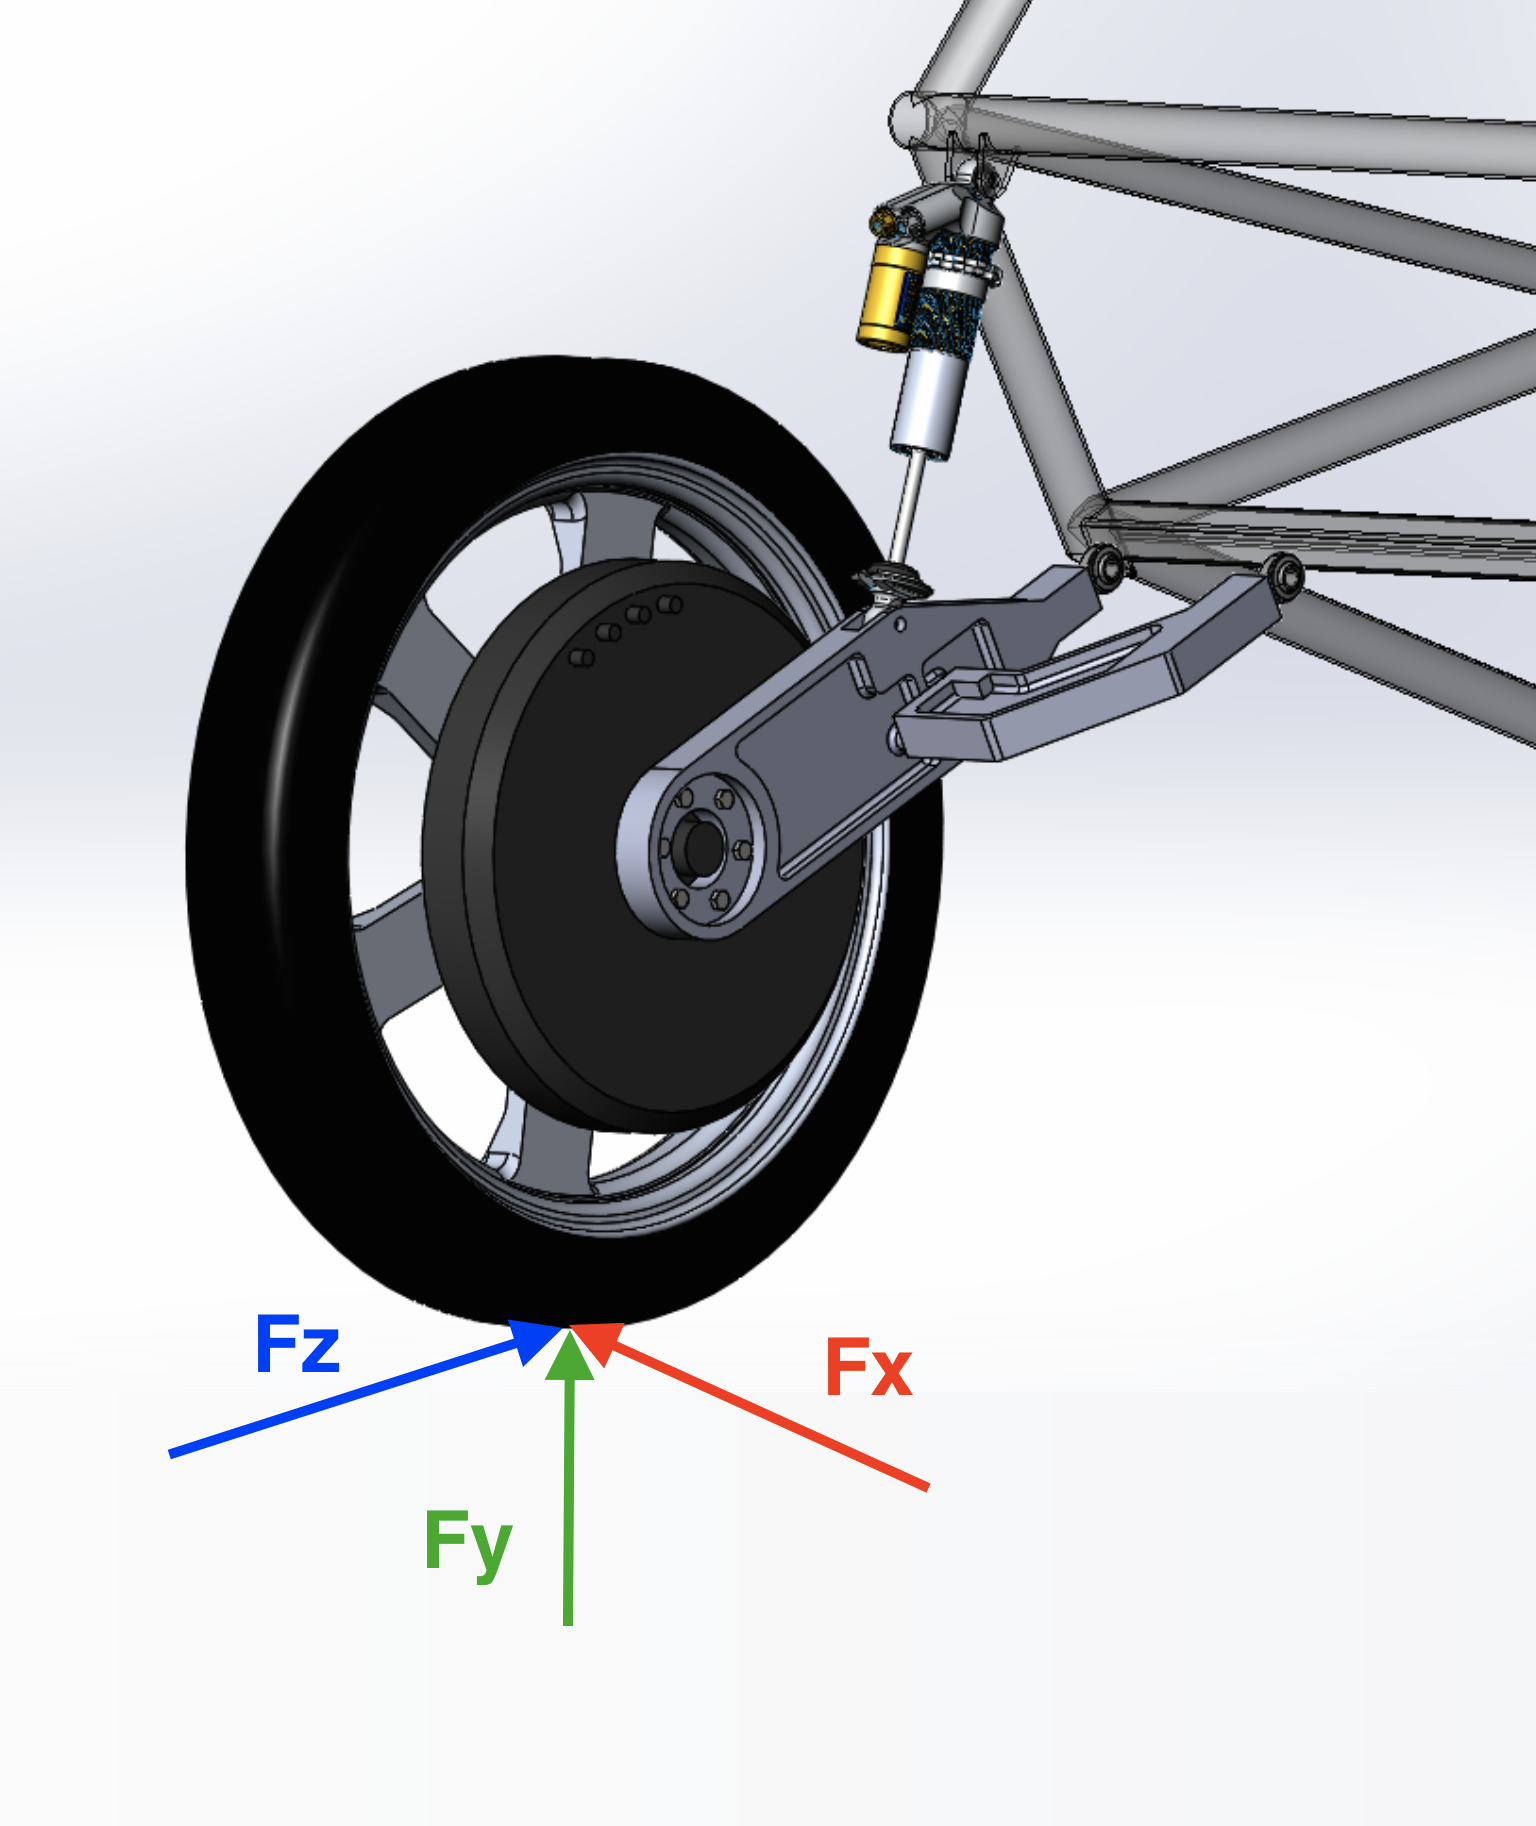
\includegraphics[height=9cm]{./LaTex/rearIsoForces.PNG}
    \end{subfigure}
    \caption{Summary of Suspension Loading Conditions}
	\label{fig:forcesSummary}
\end{figure}

Since the lateral force on each of the wheels in particular is dependent on a number of tire properties that are difficult to model (slip angle, tire pressure, etc.). It was assumed that 50\% of the net lateral force will be the maximum lateral force experienced by any one of the four wheels at a given time. 

\section{Dynamic Loading}
MSXII will be using Ohlins TTX25 dampers for both the front and rear suspension. From the Ohlins' published data, \cite{ohlins}, the maximum damping coefficient achievable is approximately 3.5kNs/m. 

% Source
\pagebreak
\bibliography{bib}{}
\bibliographystyle{plain}

% Appendix
\pagebreak
\appendix
\section{MATLAB Source Code for Simplified Model}
\label{app:simple}
\lstinputlisting[breaklines=true]{./matlab/alternativeFormulation.m}
\pagebreak
\section{MATLAB Source Code for Alternative Formulation}
\label{app:alternative}
\lstinputlisting[breaklines=true]{./matlab/simplifiedFormulation.m}

\end{document}